\documentclass[10pt, a4paper]{article}
\usepackage[utf8]{inputenc}
\usepackage[brazil]{babel}
%\usepackage{fullpage}

\usepackage[prob-boxed]{zeus}
\usetikzlibrary{patterns}

\usepackage{fullpage}
\usepackage{pgfplots}
\pgfplotsset{compat=1.15}
\usepackage{mathrsfs}
\usetikzlibrary{arrows}

\begin{document}

\begin{center}
	\textbf{Simulado OBM -- 2020.12.19}\\
\end{center}

\begin{prob}
	Qual é a maior quantidade de subconjuntos de $5$ elementos do conjunto $\{1, 2, \dots, 20\}$ que podemos escolher de modo que quaisquer dois compartilhem exatamente $1$ elemento.
\end{prob}

\begin{sk}
	Isso lembra planos projetivos finitos. Os pontos são os elementos de $\{1, 2, \dots, 20\}$ e as retas são os subconjuntos.

	\begin{center}
		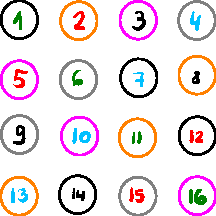
\includegraphics[height = 3cm]{fig_p1}\\
	(\emph{$17, 18, 19, 20$ estão no infinito.})
	\end{center}
\end{sk}

\begin{sol}
	A resposta é $16$. Seja $S = \{1, 2, \dots, 20\}$.

	Para todo $x \in S$, $x$ pertence a, no máximo, $4$ conjuntos. \emph{Prova a cargo do leitor.}

	Usando contagem dupla em $(x \in S, C)$, com $C$ um dos conjuntos selecionados e $x \in C$, temos que \[\#(C) \cdot 5 \le 20 \cdot 4,\]
	isto é, $\#(C) \le 16$.

	Eis um exemplo com $16$ conjuntos:
	\begin{gather*}
		\{	1,  2,  3,  4,  17 \};
	\{	5,  6,  7,  8,  17 \};
	\{	9,  10, 11, 12, 17 \};
	\{	13, 14, 15, 16, 17 \};\\
	\{	1,  5,  9,  13, 18 \};
	\{	2,  6,  10, 14, 18 \};
	\{	3,  7,  11, 15, 18 \};
	\{	4,  8,  12, 16, 18 \};\\
	\{	1,  6,  11, 16, 19 \};
	\{	2,  5,  12, 15, 19 \};
	\{	3,  8,  9,  14, 19 \};
	\{	4,  7,  10, 13, 19 \};\\
	\{	1,  4,  12, 14, 20 \};
	\{	2,  8,  11, 13, 20 \};
	\{	3,  5,  10, 16, 20 \};
	\{	4,  6,  9,  15, 20 \}.
	\end{gather*}
\end{sol}

\end{document}
